\documentclass[a4paper,12pt]{article}


\usepackage[T1]{fontenc}
\usepackage[utf8]{inputenc}
\usepackage[frenchb]{babel}

\usepackage{graphicx}

\title{Compte rendu de travaux pratiques\\ \small ou un meilleur titre}
\author{Vincent Denechaud, Olivier Maillet, Alice Odier, Félix Tora}
\date{Vendredi 24 janvier 2014}






\begin{document}

\maketitle

Voilà où on pourrait mettre l'introduction, sur les techniques MEB sans trop en faire.


\section{Les différentes sources électroniques du MEB}

Des électrons sont accélérés depuis la cathode vers l'échantillon que l'on souhaite étudier. Du fait de leur énergie cinétique, les électrons pénètrent dans la matière de l'échantillon en formant ce que l'on appelle une poire d'interaction (figure \ref{fig:poire_int}).

\begin{figure}
\centering
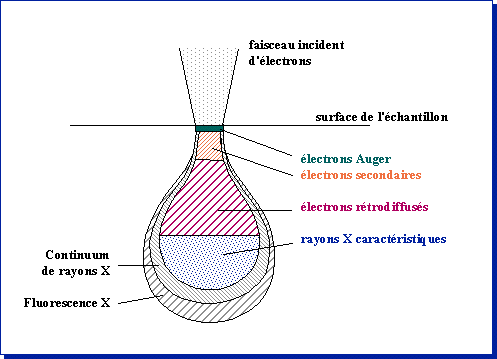
\includegraphics[width = 0.7 \textwidth]{images/poire_int.png}
\caption{Poire d'interaction}
\label{fig:poire_int}
\end{figure}


En réponse à cette excitation, la matière revient à l'équilibre en émettant du rayonnement X ainsi que des électrons, de sorte que le cortège électronique des atomes composant l'échantillon possède une configuration d'équilibre énergétique. 
On peut classer les émissions électroniques selon différentes catégories.


Lorsque les électrons viennent interagir avec l'échantillon, ils sont, pour la plupart, rétrodiffusés de manière élastique. Autrement dit, ces électrons interagissent avec les noyaux des atomes de l'échantillon de sorte à conserver leur énergie cinétique.

Ainsi, ces électrons ont une grande profondeur d'échappée et un grand libre parcours moyen dans l'échantillon.
De fait, ces électrons sont très sensibles à la composition chimique de l'échantillon, plus particulièrement, au numéro atomique Z des atomes constituant l'échantillon.
Même s'ils ont une grande longueur de pénétration, ces électrons permettent une résolution spatiale (contraste topographique) de Xnm.
\\

 

\section{On pourrait mettre une deuxième partie ici}

Sur un autre échantillon.

\vspace{5cm}

Et imaginer d'autres parties, des sous parties et des jolies images comme sur la figure \ref{fig:ni_er_amb}.

\begin{figure}
\centering
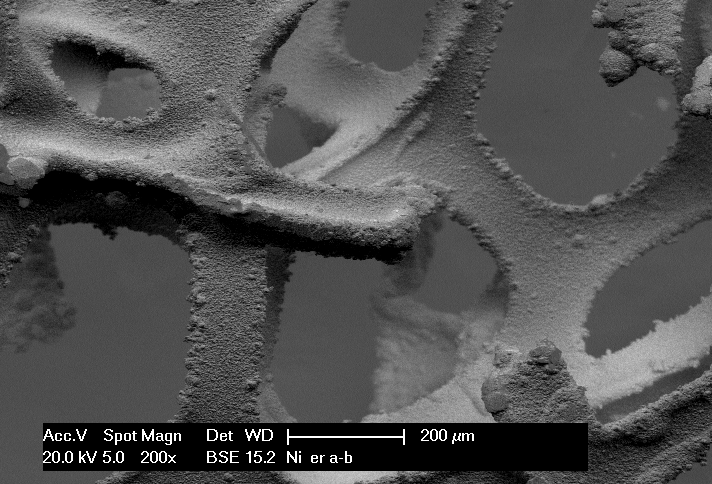
\includegraphics[width = 0.7 \textwidth]{images/ni_er_amb.png}
\caption{Avec une jolie légende en prime}
\label{fig:ni_er_amb}
\end{figure}

\section*{Conclusion}

Et puis tout à la fin on pourrait mettre une petite conclusion aux petits oignons.


\end{document}
